\chapter{Implementation}
\label{cap5}



\section{Graphical editor}\label{editor}

GEF (Graphical Editing Framework) is a Java technology, it is a part of the Eclipse framework developed by IBM.
It gives developers a full solution for graphical modeling of a Java object model, and it can be used in conjunction with other technologies such as EMF (Eclipse Modeling Framework) or GMF (Graphical Modeling Framework), to be able to gain
abstraction levels in application development.

We used EMF,GEF and GMF to develop the Pluto Graphical Editor, fully described in section \ref{plutoGraphicalEditor}.
\\

Thanks to EMF we built the abstract model of our editor, specifying all the blocks and their hierarchical structure.

Since EMF provide a \textit{code generation} feature, we easily generated the Java classes of all the blocks of the editor.
\\

We implemented the visual part of the editor using GEF.
We defined each block as a rectangle and we add connectors in order to create the final graph from which the code of the application will be generated.
\\

GMF provides a generative component and runtime infrastructure for developing graphical editors based on the Eclipse Modeling Framework (EMF) and Graphical Editing Framework (GEF).

So, through GMF the code of the final application can be generated by the graph created through blocks and connectors.

\section{Code generation}\label{codeGeneration}

%Description of the generation process of the code from diagram

Once the programmer has created the graph of the application through the Pluto Graphical Editor, he has to generate the code in order to make the Pluto Main Application behavior coherent with the graph.

This can simply be done by right clicking on the graph and choosing the "Generate code" command.

In the implementation code of the Pluto Main Application there is the \textit{MissionWorker} class, which contains two \textit{tags}.
These tags stands for the variables declaration and the instantiation of the blocks needed by the particular kind of application developed with the Pluto Graphical Editor.

The code generation process simply replaces these \textit{tags} with the variables declaration and the calls to the blocks inserted by the programmer.




\section{Object-oriented approach}\label{oomodel}

We used the Java programming language to implement both the Graphical Editor and the Main Application.
We made this choice because we are very familiar with Java, since almost every academic project we implemented in these years made use of this Object-Oriented programming language.
The Object-Oriented approach perfectly suits the Pluto model, since we have different independent entities such Drones,Missions,Trips that interact together in the execution of tasks.
\\

We decided to adopt a Model View Controller(MVC) approach, whose functioning is shown in figure \ref{fig:mvc}.
The central component of MVC, the model, captures the behavior of the application in terms of its problem domain, independent of the user interface.
The model directly manages the data, logic and rules of the application.
A view can be any output representation of information, such as a chart or a diagram; multiple views of the same information are possible.
The third part, the controller, accepts input and converts it to commands for the model or view.

A controller can send commands to the model to update the model's state.
It can also send commands to its associated view to change the view's presentation of the model.
A model notifies its associated views and controllers when there has been a change in its state. This notification allows the views to produce updated output, and the controllers to change the available set of commands.
A view requests information from the model that it uses to generate an output representation to the user.

\begin{figure}[H]
\centering
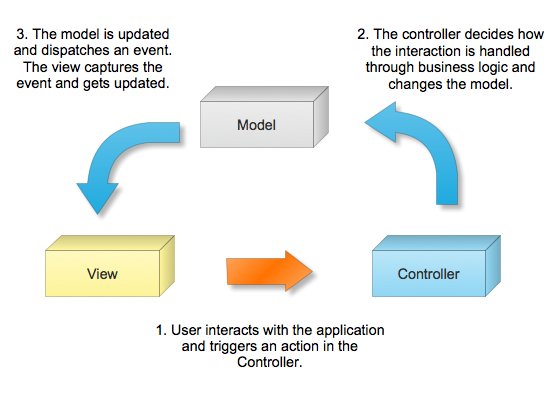
\includegraphics[width=\linewidth]
{pictures/MVC.png}
  \caption{The MVC pattern}
  \label{fig:mvc}
\end{figure}

\section{Runtime Management}\label{runtimeMng}

Description of the management of threads, pub/sub pattern and log procedures

\section{User interface}\label{interface}

We chose the Swing framework to develop the Pluto User Interface, already described in section \ref{plutoMainApp}.
We made this choice since Swing is well known to us.
Indeed we used it for the development of many academic projects, where we noticed that it allows to build graphical interface in a very fast and easy way and to add a great variety of components.
\\

Swing library is an official Java GUI toolkit released by Sun Microsystems. It is used to create Graphical user interfaces with Java.
The main characteristics of the Swing toolkit are:
\begin{itemize}
\item platform independent
\item customizable
\item extensible
\item configurable
\item lightweight
\end{itemize}

Swing is an advanced GUI toolkit. It has a rich set of widgets:
from basic widgets like buttons, labels, scrollbars to advanced like trees and tables. 
Swing itself is written in Java and is part of JFC, Java Foundation Classes: it is a collection of packages for creating full featured desktop applications.

There are basically two types of widget toolkits: \textit{Lightweight} and \textit{Heavyweight}.
A heavyweight toolkit uses OS's API to draw the widgets. For example Borland's VCL is a heavyweight toolkit since it depends on WIN32 API, the built in Windows application programming interface.
As already said, Swing is a lightweight toolkit since it paints its own widgets.

\section{The crazyflie nano-quadcopter}\label{crazyflie}

For the concrete actuation of the sensing tasks required by each application, we chose the Crazyflie Nano-Quadcopter, shown in figure \ref{fig:crazyflie}.


\begin{figure}[H]
\centering
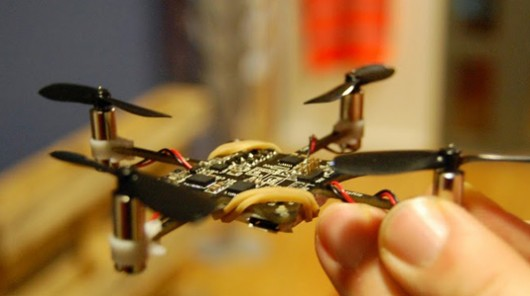
\includegraphics[width=\linewidth]
{pictures/crazyflie.jpg}
  \caption{The Crazyflie Nano-Quadcopter}
  \label{fig:crazyflie}
\end{figure}

The Crazyflie is a tiny quadcopter often referred to as a nano-quad, built using the PCB itself as the frame,developed solely by open source tools. The Crazyflie specs are the following:


\begin{itemize}
\item {Small and lightweight, around 19g and about 90mm motor to motor
}
\item {Flight time up to 7 minutes with standard 170mAh Li-Po battery
}
\item {Standard micro-USB connector for charging which takes 20min for the stock 170mAh Li-Po battery
}
\item {On-board low-energy radio@1mW based on the nRF24L01+ chip. Up to 80m range (environment dependent) when using the Crazyradio USB dongle}
\item{Radio bootloader which enables wireless update of the firmware
}
\item{Powerful 32 bit MCU: STM32F103CB @ 72 MHz (128kb flash, 20kb RAM)
}
\item{3-axis high-performance MEMs gyros with 3-axis accelerometer: Invensense MPU-6050
}
\item{Available footprints to manually solder magnetometer HMC5883L/HMC5983 or/and barometer MS5611
}
\item{4-layer low noise PCB design with separate voltage regulators for digital and analog supply
}
\end{itemize}

To concretely control the Crazyflie, there is a Python library which gives high level functions and hides the details.
We used a particular API to send the control command: 
\\

\begin{lstlisting}
	send_setpoint(roll, pitch, yaw, thrust)
\end{lstlisting}

The arguments roll/pitch/yaw/trust is the new set-points that should be sent to the copter.
For example, to send a new control set-point:
\\

\begin{lstlisting}
	 roll    = 0.0
    pitch   = 0.0
    yawrate = 0
    thrust  = 0
    crazyflie.commander.send_setpoint(roll, pitch, yawrate, thrust)
\end{lstlisting}

Changing the \textit{roll} and \textit{pitch} will make the quadcopter tilt to the sides and thus change the direction that it's moving in.
Changing the \textit{yaw} will make the quadcopter spin.
The thrust is used to control the altitude of the quadcopter.

By dynamically adjusting these four parameters we can make the Crazyflies move to the locations specified by the user through the Pluto User Interface.


